\documentclass{report}

\input{../template/preamble}
\input{../template/macros}
\input{../template/letterfonts}

\newcolumntype{Y}{>{\centering\arraybackslash}X}

\title{\Huge{Magnetism}\\Semester 5}
\author{Ahmad Abu Zainab}
\date{}

\begin{document}

\maketitle
\newpage% or \cleardoublepage
% \pdfbookmark[<level>]{<title>}{<dest>}
\pdfbookmark[section]{\contentsname}{toc}
\tableofcontents
\pagebreak

\chapter{Electromagnetic Waves}

Electromagnetic waves are waves that are created by oscillating electric and magnetic fields. The electric and magnetic fields are perpendicular to each other and to the direction of propagation of the wave.
They travel at a speed of $c=299792458$ \unit{m/s} in a vacuum. The frequency of the wave is given by $f=\frac{c}{\lambda}$ where $\lambda$ is the wavelength of the wave.

The wavelength is the distance between two consecutive peaks of the wave.

\begin{figure}[ht]
	\centering
	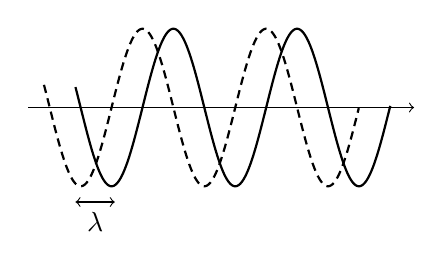
\begin{tikzpicture}[domain=-4:0]
		\draw[->] (-4.2,0) -- (0.7,0);

		\draw[smooth,thick, samples=1000, densely dashed]   plot (\x,{sin(4*\x r)});
		\draw[smooth,thick, samples=1000, domain=-3.6:0.4]   plot (\x,{sin(4*\x r - 90)});
		\draw[<->] (-3.6,-1.2) -- (-3.1,-1.2) ;
		\draw (-3.35,-1.2) node[below] {$\lambda$};
	\end{tikzpicture}
\end{figure}

The wave moves a distance $x$ in a time $t$ with a speed
\[
	v = \frac{x}{t} = \frac{\omega}{k} = \frac{\lambda}{T} = \lambda f
	.\]

\[
	\lambda = \frac{2\pi}{f}
	.\]

The equation of the wave is given by

\[
	y = A\sin \lt( \omega t - kx + \phi \rt)
	.\]

The intensity of the wave is given by

\[
	I = \frac{P}{4 \pi r^2}
	.\]

\subsection{Poynting Vector}

The Poynting vector is a vector that represents the energy flux of the wave. It is given by

\[
	\va{S} = \frac{1}{\mu_0}\va{E} \times \va{B}
	.\]

However, since $\va{B}$ are perpendicular to $\va{E}$ then

\[
	S = \frac{1}{\mu_0}EB
	.\]

and since

\[
	c = \frac{E}{B}
	.\]

then

\[
	S = \frac{c}{\mu_0}B^2 = \frac{1}{c\mu_0}E^2
	.\]

\subsection{Maxwell's Equations}

\begin{align*}
	\pdv{\va{E}}{x} & = - \pdv{\va{B}}{t}                     \\
	\pdv{\va{B}}{x} & = - \varepsilon_0 \mu_0 \pdv{\va{E}}{t}
\end{align*}

\chapter{Optics}

The equation of an EM wave is given by

\[
	\va{E} = E_0 \sin \lt( \omega t - kx \rt) \vu{\jmath}
	.\]

Noting that electric field typically have all directions, whenever an non-polarised electric field hits a polariser, only the electric field components that are along the line of polarization are allowed to pass while all others are absorbed. If the electric field direction is perpendicular to the line of polarization then it is entirely absorbed while the electric field vectors that have an angle $\theta <\pi /2$ then only the projection of that vector on the polarization line will not be absorbed.

Given a polariser with angle $ \alpha $ then the electric field $\va{E } $ hitting that polariser has an equation

\[
	\va{E} = \underbrace{E \sin \alpha\vu{u}_1}_{\text{transmitted}} + \underbrace{E\cos \alpha\vu{u}_2}_{\text{absorbed}}
	.\]

\subsection{Reflection}

The angle of incidence is equal to the angle of reflection.

\[
	\theta_i = \theta_r
	.\]

\begin{figure}[H]
	\centering
	\begin{tikzpicture}
		\draw[->,thin] (-4,0) -- (4,0);
		\draw[->,thin] (0,0) -- (0,4);
		\draw[-{Latex},thick] (0,0) -- (2,2) node[above] {$\va{E}_i$};
		\draw[-{Latex},thick] (-2,2) node[above] {$\va{E}_r$} -- (0,0);
		\draw (0,0.5) arc (90:135:0.5) node[midway,above] {$\theta_i$};
		\draw (0,0.5) arc (90:45:0.5) node[midway,above] {$\theta_r$};
	\end{tikzpicture}
\end{figure}


\subsection{Refraction}
Snell's law
\[
	n_1\sin \theta_1 = n_2\sin \theta_2
	.\]

\begin{figure}[H]
	\centering
	\begin{tikzpicture}
		\draw[thin] (-3,0) -- (3,0);
		\draw[thin, dashed] (0,-2.7) -- (0,2.7);
		\draw[-{Latex},thick] (-2,2) -- (0,0);
		\draw[-{Latex},thick] (0,0) -- (1,-3);
		% Draw the angle 
		\draw (0,0.6) arc (90:135:0.6) node[midway,above] {$\theta_1$};
		\draw (0,-0.6) arc (-90:-73:0.6) node[midway,below] {$\theta_2$};
		\draw (3,1) node[above] {$n_1$};
		\draw (3,-1) node[above] {$n_2$};
	\end{tikzpicture}
\end{figure}

This implies that if $n_1 < n_2$ then $\theta_1 > \theta_2$.


\dfn{Critical Angle}{
	The critical angle the maximum angle of refraction where the refracted ray goes back in the incident medium

	\[
		\theta_c = \sin^{-1} \lt( \frac{n_2}{n_1} \rt)
		.\]
	\begin{figure}[H]
		\centering
		\begin{tikzpicture}
			\begin{scope}[xshift=-3cm, scale=0.75]
				\draw[thin] (-3,0) -- (3,0);
				\draw[thin, dashed] (0,-2.7) -- (0,2.7);

				\draw[-{Latex},thick] (-1.5,-1.5) -- (0,0);
				\draw[-{Latex},thick] (0,0) -- (2,0);

				\draw (2,1) node[above] {$\theta_1=\theta_c$};
				\draw (2,-1) node[above] {$\theta_2=\ang{90}$};

				\draw (0,-0.5) arc (-90:-135:0.5) node[midway,below] {$\theta_1$};
				\draw (0,0.5) arc (90:0:0.5) node[midway,above] {$\theta_2$};
			\end{scope}
			\begin{scope}[xshift=3cm, scale=0.75]
				\draw[thin] (-3,0) -- (3,0);
				\draw[thin, dashed] (0,-2.7) -- (0,2.7);

				\draw[-{Latex},thick] (-2.5,-1) -- (0,0);
				\draw[-{Latex},thick] (0,0) -- (2.5,-1);

				\draw (-2,1) node[above] {$\theta_1>\theta_c$};

				\draw (0,-0.5) arc (-90:-158.2:0.5) node[midway,below] {$\theta_1$};
				\draw (0,-0.5) arc (-90:-21.8:0.5) node[midway,below] {$\theta_2$};
			\end{scope}

		\end{tikzpicture}
	\end{figure}
}

\[
	v = \frac{c}{n}
	.\]

\begin{align*}
	\text{Speed of light in a medium} & = \frac{1}{\sqrt{\mu \varepsilon}}     \\
	\text{Speed of light in a vacuum} & = \frac{1}{\sqrt{\mu_0 \varepsilon_0}} \\
	\text{Refractive index}           & = \sqrt{\mu_r \varepsilon_r}
\end{align*}


\[
	\frac{n_1}{n_2} =\frac{v_2}{v_1}
	.\]

\section{Young's Double Slit Experiment}

\[
	d\sin \theta = m\lambda
	.\]

\[
	\Delta x = \frac{m\lambda L}{d}
	.\]

Bright fringes are where the path difference is an integer multiple of the wavelength.
\[
	x = \frac{m\lambda L}{d}
	.\]

Dark fringes are where the path difference is an odd multiple of half the wavelength.

\[
	x = \frac{\lt( 2m+1 \rt)\lambda L}{2d}
	.\]

Where $m$ is an integer, $d$ is the distance between the slits, $\lambda$ is the wavelength of the light, $L$ is the distance between the slits and the screen, and $x$ is the distance between the central bright fringe and the $m$th bright fringe.

\section{Diffraction Grating}

\[
	\sin \theta_1 = \frac{\lambda}{a}
	.\]

\[
	\sin \theta_n = n\frac{\lambda}{d}
	.\]

\chapter{Transmission Lines}

\section{The Phasor}

The phasor is a complex number that represents the amplitude and phase of a sinusoidal function. It is given by 2 forms

\[
	\text{Rectangular form} = A\cos \lt( \omega t + \varphi \rt) + jA\sin \lt( \omega t + \varphi \rt)
	.\]

\[
	\text{Polar form} = Ae^{j\lt( \omega t + \varphi \rt)} = A \phase{\omega t + \varphi}
	.\]

\section{The Role of Wavelength}

In a transmission line, the wavelength of the signal can affect the impedance of the line. The voltage at the source ($V_{AA'}$) is given by

\[
	V_{AA'} = V_0 \cos \omega t
	.\]

The voltage at the load ($V_{BB'}$) (assuming no losses across the transmission line) is given by

\[
	V_{BB'} = V_0 \cos \lt( \omega t - \varphi_0 \rt)
	.\]

\[
	\varphi_0 = \frac{\omega l}{c}
	.\]

\section{TL lumped element model}

We can model a transmission line using a series of resistors, inductors, and capacitors. The model is given by 4 parameters

\begin{align*}
	R' & = \text{Resistance per unit length } [\unit{\ohm\per\meter}]      \\
	L' & = \text{Inductance per unit length } [\unit{\henry\per\meter}]    \\
	C' & = \text{Capacitance per unit length } [\unit{\farad\per\meter}]   \\
	G' & = \text{Conductance per unit length } [\unit{\siemens\per\meter}]
\end{align*}

{
\renewcommand{\arraystretch}{2.5}
\everymath{\displaystyle}
\begin{table}[H]
	\centering
	\begin{tabularx}{\linewidth}{|c|YYYc|}
		\hline
		\textbf{Parameter} & \textbf{Coaxial}                                       & \textbf{Two-Wire}                                             & \textbf{Parallel-Plate}   & \textbf{Unit}               \\
		\hline
		$R'$               & $\frac{R_s}{2\pi} \lt( \frac{1}{a} + \frac{1}{b} \rt)$ & $\frac{2R_s}{\pi d}$                                          & $\frac{2R_s}{w}$          & $\unit{\ohm\per\meter}$     \\
		$L'$               & $\frac{\mu}{2\pi}\ln b/a $                             & $\frac{\mu}{\pi}\ln\lt[ (D/d)+\sqrt{(D/d)^2-1} \rt]$          & $\frac{\mu h}{w}$         & $\unit{\henry\per\meter}$   \\
		$G'$               & $\frac{2\pi \sigma}{\ln b/a}$                          & $\frac{\pi \sigma}{\ln\lt[ (D/d)+\sqrt{(D/d)^2-1} \rt]}$      & $\frac{\sigma w}{h}$      & $\unit{\siemens\per\meter}$ \\
		$C'$               & $\frac{2\pi \varepsilon}{\ln b/a}$                     & $\frac{\pi \varepsilon}{\ln\lt[ (D/d)+\sqrt{(D/d)^2-1} \rt]}$ & $\frac{\varepsilon w}{h}$ & $\unit{\farad\per\meter}$   \\
		\hline
	\end{tabularx}
\end{table}
}
Where $\mu$, $\varepsilon$, and $\sigma$ are the permeability, permittivity, and conductivity of the medium respectively. $R_s=\sqrt{\pi f \mu_c/\sigma_c}$ is the resistance of the conductor, $a$ is the radius of the inner conductor, $b$ is the radius of the outer conductor, $D$ is the distance between the two wires, $d$ is the diameter of the wire, $w$ is the width of the plate, and $h$ is the height of the plate.\\

\section{The Telegrapher's Equations}

The wave equation is given by

\[
	\dv[2]{\tilde{V}(z)}{z} - \lt( R' + j\omega L' \rt) \lt( G' + j\omega C' \rt) \tilde{V}(z) = 0
	.\]

Thus, we define the complex propagation constant $\gamma$ as
\[
	\gamma = \alpha + j\beta
	.\]

Where $\alpha$ is the attenuation constant and $\beta$ is the phase constant.

\begin{align*}
	\alpha & = \Re \lt( \gamma \rt)\quad [\unit{\neper\per\meter}]  \\
	\beta  & = \Im \lt( \gamma \rt)\quad [\unit{\radian\per\meter}]
\end{align*}

In uncoupled form, the telegrapher's equations are given by

\begin{align*}
	\dv[2]{\tilde{V}(z)}{z} - \gamma^2 \tilde{V}(z) & = 0 \\
	\dv[2]{\tilde{I}(z)}{z} - \gamma^2 \tilde{I}(z) & = 0
\end{align*}

The general solution to the wave equation is given by

\begin{align*}
	\tilde{V}(z) & = {V_0}^+ e^{-\gamma z} + {V_0}^- e^{\gamma z} \\
	\tilde{I}(z) & = {I_0}^+ e^{-\gamma z} + {I_0}^- e^{\gamma z}
\end{align*}

Where ${V_0}^+$ and ${I_0}^+$ are the incident voltage and current respectively and ${V_0}^-$ and ${I_0}^-$ are the reflected voltage and current respectively.\\

The characteristic impedance of the transmission line is given by

\[
	Z_0 = \frac{R' + j\omega L'}{\gamma} = \sqrt{\frac{R' + j\omega L'}{G' + j\omega C'}} \quad [\unit{\ohm}]
	.\]

\section{Lossless Transmission Line}

In a lossless transmission line, the resistance and conductance per unit length are zero. I.E. $R'\ll \omega L'$ and $G'\ll \omega C'$. Thus, the characteristic impedance is given by

\begin{align*}
	\alpha  & = 0                                                                                                               \\
	\beta   & = \omega \sqrt{L'C'} = \omega \sqrt{\mu\varepsilon}                                                               \\
	Z_0     & = \sqrt{\frac{L'}{C'}}                                                                                            \\
	\lambda & = \frac{2\pi}{\beta} = \frac{2\pi}{\omega \sqrt{L'C'}}                                                            \\
	u_p     & = \frac{\omega}{\beta} = \frac{1}{\sqrt{L'C'}} = \frac{1}{\sqrt{\mu\varepsilon}} \quad [\unit{\meter\per\second}]
\end{align*}

\section{Voltage Reflection Coefficient}

The voltage reflection coefficient is given by

\begin{align*}
	\Gamma & = \frac{{V_0}^-}{{V_0}^+}     \\
	       & = \frac{Z_L - Z_0}{Z_L + Z_0} \\
	       & = \frac{z_L -1}{z_L + 1}
\end{align*}

Where $z_L = Z_L/Z_0$ is the load impedance in terms of the characteristic impedance.\\

We represent the voltage and current on the transmission line as

\begin{align*}
	\tilde{V}(z) & = {V_0}^+ \lt( e^{-j\beta z} + \Gamma e^{j\beta z} \rt)             \\
	\tilde{I}(z) & = \frac{{V_0}^+}{Z_0} \lt( e^{-j\beta z} - \Gamma e^{j\beta z} \rt)
\end{align*}

\[
	{V_0}^- = \Gamma {V_0}^+
	.\]

\section{Special Line Conditions}

\begin{enumerate}
	\ii Matched Line: $Z_L = Z_0 \Rightarrow \Gamma = 0$ $V_\text{ref} = 0$
	\ii Open Circuit: $Z_L = \infty \Rightarrow \Gamma = 1$ $V_\text{ref} = V_\text{inc}$
	\ii Short Circuit: $Z_L = 0 \Rightarrow \Gamma = -1$ $V_\text{ref} = -V_\text{inc}$
\end{enumerate}

{
\renewcommand{\arraystretch}{2.5}
\everymath{\displaystyle}
\begin{table}[H]
	\centering
	\begin{tabularx}{0.8\linewidth}{|c|YY|}
		\hline
		\textbf{Load}              & $\bm{|\Gamma|}$                                       & $\bm{\theta_r}$                                                          \\
		\hline
		$Z_L = (r + jx)Z_0$        & $\lt[ \frac{(r-1)^2 + x^2}{(r+1)^2 + x^2} \rt]^{1/2}$ & $\tan^{-1} \lt( \frac{x}{r-1} \rt) - \tan^{-1} \lt( \frac{x}{r+1} \rt) $ \\
		$Z_L = Z_0$                & 0                                                     & Irrelevant                                                               \\
		(short)                    & 1                                                     & $\pm\pi$ (phase opposite)                                                \\
		(open)                     & 1                                                     & 0                                                                        \\
		$jX = j\omega L$           & 1                                                     & $\pm\pi - 2\tan^{-1}x$                                                   \\
		$jX = -\frac{j}{\omega C}$ & 1                                                     & $\pm 2\tan^{-1}x$                                                        \\
		\hline
	\end{tabularx}
\end{table}
}

% \section{Standing Waves} 
%
% Standing waves are waves that do not propagate. They are formed when two waves of the same frequency and amplitude travel in opposite directions. The equation of a standing wave is given by 
%
% \[
%     V(z,t) = V_0 \cos \lt( \omega t \rt) \lt[ e^{-j\beta z} + \Gamma e^{j\beta z} \rt]
%     .\]

\end{document}
